\documentclass[12pt, french]{article}

\usepackage{fancyhdr, fancybox, lastpage , xcolor, 
            enumerate,
            amsmath,fontenc, mhchem}
\usepackage{wrapfig}
\usepackage[most]{tcolorbox}
\usepackage[a4paper, margin={0.3in, .75in}]{geometry}
\usepackage{multirow}

\pagestyle{fancy}
\renewcommand\headrulewidth{1pt}
\renewcommand\footrulewidth{1pt}
\fancyhf{}
\rhead{ \em{Zakaria Haouzan}}
\lhead[C]{\em{1ére année baccalauréat Sciences Mathématiques}}
\chead[C]{}
\rfoot[C]{}
\lfoot[R]{}
\cfoot[]{\em{Page \thepage / \pageref{LastPage}}}


\newtcolorbox{Box2}[2][]{
                lower separated=false,
                colback=white,
colframe=white!20!black,fonttitle=\bfseries,
colbacktitle=white!30!gray,
coltitle=black,
enhanced,
attach boxed title to top left={yshift=-0.1in,xshift=0.15in},
title=#2,#1}


\begin{document}
\begin{center}

   \shadowbox {\bf{Dosages (ou titrages) directs}}
\end{center}


%%_________________________Exercice ! :"_________________________Exercice
   \begin{Box2}{Exercice 1 :dosage d'une solution de Tarnier par une solution de thiosulfate de sodium} 
      Pour déterminer la concentration $C_1$ en diiode ${I_2}_{(aq)}$ d’une solution de Tarnier, on dose un volume
      $V_1 =25,0 mL$ de solution de Tarnier par une solution de thiosulfate de sodium $(2{Na^+}_{(aq)} + {S_2O_3^{2-}}_{(aq)})$ de
concentration $C_2=0,0200 mol/L$.
      \\Données : ${I_2}_{(aq)} / {I^-}_{(aq)}$ et ${S_4O_6^{2-}}_{(aq)} / {S_2O_3^{2-}}_{(aq)}$

      Le volume versé à l’équivalence est égal à $V_{2E}=12,1 mL$.
\\1. Etablir l’équation de la réaction de dosage.
\\2. Etablir un tableau d’avancement.
      \\3. En déduire une relation entre $n(I_2)$ et $n(S_2O_3^{2-})$.
\\4. Déterminer la concentration $C_1$ du diiode.


   \end{Box2}

%%_________________________Exercice !2 :"_________________________Exercice
\begin{Box2}{Exercice 2 :Titrage conductimétrique 
 }\begin{wrapfigure}{r}{0.4\textwidth}
  \begin{center}
    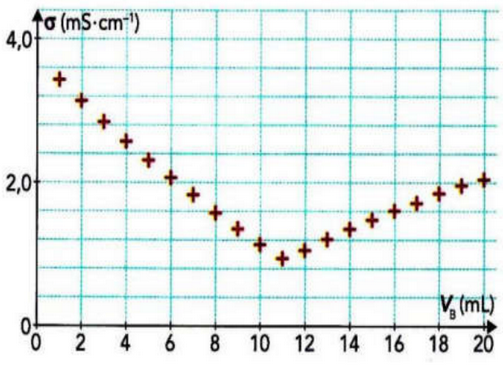
\includegraphics[width=0.4\textwidth]{./Screenshot from 2022-05-11 17-55-37.png}
  \end{center}
\end{wrapfigure}



   On dose, par titrage conductimétrique, une solution $S_A$ d'acide chlorhydrique, ${H_3O^+}_{(aq)} + {Cl^-}_{(aq)}$, par une solution
$S_B$ d'hydroxyde de sodium, ${Na^+}_{(aq)} + {HO^-}_{(aq)}$. L'équation de la réaction de titrage est :
   \\$\ce{{H_3O^+}_{(aq)} + {HO^-}_{(aq)} -> 2{H_2O}_{(l)}}$

Le suivi du titrage par conductimétrie permet de tracer le graphe $\sigma = f(V_B)$ ci-dessous :

   1. Faire un schéma légendé du dispositif de titrage.

2. Déterminer le volume équivalent $V_E$ du titrage. On néglige la dilution lors du titrage.

3. On se place avant l'équivalence.

      3.1. Quel est le réactif limitant?

      3.2. La concentration en ions chlorure varie-t-elle au cours du
titrage?

      3.3. L'expression de la conductivité $\sigma$ de la solution contenue
   dans le bécher est : $\sigma = \lambda(H_3O^+).[H_3O^+]$ Sachant que $\lambda( H_3O^+> \lambda( Na^+)$, justifier l'évolution de la conductivité $\sigma$ avant l'équivalence.

   4. On se place maintenant après l'équivalence.

   4.1. Quel est le réactif limitant?

   4.2. Établir l'expression de la conductivité $\sigma$

   4.3. Justifier l'évolution de la conductivité de la solution
contenue dans le bécher après l'équivalence du titrage.
\end{Box2}
%%_________________________Exercice 4 : _________________________Exercice
\begin{Box2}{Exercice 3 : la masse de sulfate de fer(II)}
On pèse 1,0 g de sulfate de fer(II) impur. On le dissout dans un peu d'eau et on acidifie la solution à l'aide
d'acide sulfurique et on ajoute la solution de permanganate. 

   La coloration rose persistante est obtenue
lorsque nous avons ajouté 24,5 mL d'une solution de permanganate de potassium 0,025 mol/L.

   Calculez la masse de sulfate de fer(II) dans 1,0 g de sulfate de fer impur.
\end{Box2}


%%_________________________Exercice 3 : _________________________Exercice
\begin{Box2}{Exercice 4 :  Vinaigre(acide acétique $(CH_3COOH)$ ) }
On désire par cet exercice déterminer la concentration molaire $C_0$ en acide acétique $(CH_3COOH)$ du vinaigre du commerce, on prépare alors une solution diluée $100$ fois de concentration $C_A$.

Ensuite, on prélève un volume $V_A = 10,0 mL$ de cette solution diluée que l'on dose par une solution d'hydroxyde de
sodium $(Na^+ + HO^-)$ de concentration $C_B = 10.10^{-3} mol.L^{-1}$.

   Le volume de réactif titrant (hydroxyde de sodium) versé à l'équivalence vaut $V_{BE} = 9,7 mL.$

1. Identifier les deux couples acido-basiques mis en jeu dans ce titrage et écrire l'équation de la réaction.

2. Expliquer à quoi correspond l'équivalence.

3. Le titrage est suivi par une mesure de la conductivité de la solution dosée.

3.1. Expliquer pourquoi la conductivité augmente doucement du début du titrage jusqu'à l'équivalence.

3.2. Expliquer pourquoi la conductivité augmente fortement après l'équivalence.

   4. En utilisant un tableau d’avancement simplifié, trouver la relation entre la quantité de matière d'acide
acétique titrée $n_A$ et la quantité de matière d'hydroxyde de sodium versé $n_B$ à l'équivalence ?

5. Calculer la concentration en acide acétique $C_A$ de la solution de vinaigre diluée.

6. En déduire la concentration $C_0$ en acide acétique du vinaigre commercial.
\end{Box2}

%\vspace{3cm}
\begin{center}
   \Large{ \em{Exercices Supplémentaires}}
\end{center}
%%_________________________Exercice 6 : _________________________Exercice

%%_________________________Exercice 7 : _________________________Exercice

\begin{Box2}{Exercice 5 :dosage du permanganate de potassium }
 
   On prépare une solution $S_1$ de permanganate de potassium $(K^+_{(aq)} + MnO^-_{4 (aq)})$ de coloration violette en dissolvant une
   masse m de $KMnO_{4 (s)}$ dans un volume $V=100mL$ d'eau,( acidifiée par quelques gouttes d'acide sulfurique).

Pour déterminer la concentration de la solution $S_1$, on prélève à l'aide d'une pipette un volume $V_1=10mL$ de cette solution qu'on introduit dans un bécher et on lui ajoute progressivement une solution $S_2$ d'acide oxalique $H_2C_2O_4$ de
concentration $C_2=0,4mol/L$.

1. Comment s'appelle cette étude expérimentale qui a pour objet la détermination de la concentration de la solution $S_1$ ?

2. Donner le schéma du dispositif expérimental utilisé dans cette étude en nommant ses différents constituants.

3. Comment s'appelle la solution dont on doit déterminer la concentration ? et comment s'appelle la solution ajouté?

4. Ecrire l'équation de la réaction qui se produit durant cette étude sachant que:
l'acide oxalique est réducteur du couple $CO_2/H_2C_2O_4$ et l' ion permanganate est oxydant du couple $MnO_4^-/Mn^{2+}$.

5. Construire le tableau d'avancement de cette réaction et en déduire la relation d'équivalence.

6. Comment repérer l'équivalence dans cette étude?

   7. Quel est le réactif limitant avant l'équivalence et quel est celui limitant après l'équivalence?

   8. Sachant que le volume ajouté à l'équivalence est : $V_{2eq}=12,5mL$, déterminer la concentration $C_1$ de la solution $S_1$.

9. Déterminer la masse m utilisée pour préparer la solution $S_1$.

10. Pour diluer la solution $S_1$ , quel volume d'eau doit- on ajouter à $90mL$ de la solution $S_1$ pour que sa concentration devient $ C'=0.1 mol/L $?

on donne : g=10N/kg - M(K)=39,1g/mol - M(Mn)=54,9g/mol - M(O)=16g/mol
\end{Box2}

%%___


\end{document}
